\ofjob{Marksman}
{
	\ofquote{"I play the leading man; who else?"\\}{Balthier}\\\\
	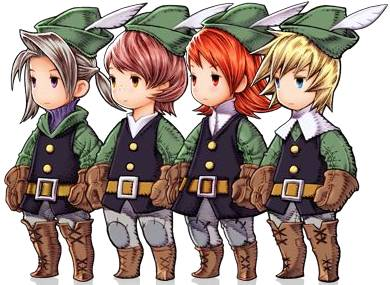
\includegraphics[width=\columnwidth]{./art/jobs/marksman.jpg}\ofrow
	\accf{Marksmen} are experts of all kinds of ranged weapons that strike from great distance. 
	Skilled Marksmen can see through their enemies, allowing them to know a target's strengths and weaknesses. 
	Therefore they can not only deal significant ranged damage, but also disable enemies with special techniques.
}
{Bow or Gun}{Light Armor}{
	Level 1: & HP +19 & MP~+17 & AGI~+2 & STR +1 \\
	Level 2: & HP~+10  & MP~+10 & DEF~+1 \\
	Level 3: & \multicolumn{3}{l}{Archetype Attribute Bonus}  \\
	Level 4: & HP~+5  & MP~+5  & STR~+2 & RES~+1 \\
	Level 5: & HP~+5  & MP~+10 & DEF~+1 & RES~+1  \\
	Level 6: & HP~+10 & MP~+10 & RES~+1 &        \\
	Level 7: & HP~+5  & MP~+10 & STR~+1 & RES~+1 \\
	Level 8: & HP~+10  & MP~+5 & DEF~+2 		  \\
	Level 9: & HP~+5  & MP~+10 & RES~+1 & STR~+1 \\
	Level 10:& HP~+10 & MP~+10 & STR~+1 &        
}{
	\ofjobtech{Libra}{4}{0r}{Single}{5u}{You analyse the target thoroughly and know his Resiliences, Weaknesses, Immunities, as well as his current HP and MP.}{}{1}\ofabilitygap
	\ofjobtech{Big Shot}{6}{0r}{Single}{Weapon}{Make an Attack on the target. If you hit, the damage dealt ignores the target's DEF.}{}{2}\ofabilitygap
	\ofjobtech{Quick Shot}{8}{0r}{Single}{Weapon}{You make an Attack after which you can immediately begin using another Ability in the same turn.}{}{6}\ofabilitygap
	\ofjobtech{Smoke Bomb}{10}{0r}{3u}{8u}{You create an Obscure Field in the target area that lasts for 3 rounds.}{}{8}\ofabilitygap
	\ofjobtech{Barrage}{22}{1r}{Single}{Self}{For the next 3 rounds you gain Haste and EnSTR. In addition, all of your Attacks and Techs which target a single enemy instead affect all enemies within 2u of the chosen target.
	}{}{10}
}{
	\ofarchetypet{Ranger}
	{HP~+13 & MP~+12 & DEF~+2}
	{\ofarchetypetecha{Lay Trap}{4}{0r}{1u}{Self}{You set a trap where you are standing. An enemy that walks over it makes a DC 9 check and suffers 1d damage and Immobile for 1 round upon failure. The trap disappears once it is activated.}{\immobile}}
	{\ofarchetypepassive{Recoil}{Whenever you make a successful Attack, you can immediately move 1u in any direction.}}
	{\ofarchetypereaction{Magic Evade}{You can evade Magic by passing an evasion check. When you evade an Attack or Magic, you also regain an amount of MP equal to your current Level.}}
	{\ofarchetypetechb{Poison Ammo}{10}{0r}{Single}{Weapon}{Make an Attack on the target. If you hit, the damage dealt is magical and the target makes a DC 8 check. Upon failure, he suffers Poison, DeSTR and DeDEF for 3 rounds.}{\poison\destr\dedef}}
}{
	\ofarchetypet{Sniper}
	{HP~+5 & MP~+15 & STR~+3}
	{\ofarchetypetecha{Pierceshot}{6}{0r}{10u (line)}{Self}{Make an Attack against all targets in a line, by making one damage roll that applies to everyone that fails to evade.}{}}
	{\ofarchetypepassive{Concentrate}{Whenever you Attack an enemy, he has Disadvantage on the evasion check.}}
	{\ofarchetypereaction{Camouflage}{Whenever you end a turn in which you have not moved, you gain Blink until the start of your next turn.}}
	{\ofarchetypetechb{Aim}{8}{0r}{Single}{Weapon}{Make an Attack on the target and choose one of the following spots to inflict an additional effect if you hit:\\ \acc{Head:} the target's evasion DC is reduced by 2, but if you hit you score a Critical Hit.\\ \acc{Heart:} MP is reduced by same amount as HP.\\ \acc{Leg:} the target suffers Immobile for 1 round.}{}}
}